\chapter{Design considerations for a heterodyne interferometer}
\label{ch:DesignConsiderations}


\section{Geometric considerations}


\subsection{Finite sampling-volume effects}
\label{sec:DesignConsiderations:geometric:finite_sampling_volume}
Practically speaking, detection is always effected
via detector elements of \emph{finite} size,
with the output of each detector element
corresponding to the incident intensity
\emph{averaged} over the element's active area.
This averaging acts as a low-pass filter in the spatial domain and
is referred to as the finite sampling volume effect~\cite{bravenec_rsi95}.

Finite sampling-volume effects dictate
a heterodyne interferometer's wavenumber response~\cite{davis_rsi16}.
To see this, assume that measurements
are made with the detector array shown in
Fig.~\ref{fig:DesignConsiderations:detector_array}.
Let the $j$\ts{th} detector element $D_j$ be centered on $x_{\image,j}$
and $y_{\image} = 0$;
the fluctuating baseband-equivalent optical power
incident on this element is then
\begin{align}
  \tilde{P}_{IQ,j}(t)
  &=
  \int_{D_j} \tilde{I}_{IQ}(\vect{r}_{\image}, t) dA
  \notag \\
  &\approx
  I_G(\vect{r}_{\image,j}) s_y
  \int_{x_{\image,j} - s_x / 2}^{x_{\image,j} + s_x / 2}
  \tilde{\phi}(x_{\image}, t)
  dx_{\image},
  \label{eq:DesignConsiderations:fluctuating_baseband_equivalent_optical_power_per_element_v1}
\end{align}
where $\tilde{I}_{IQ}(\vect{r}_{\image}, t)$
is the fluctuating baseband-equivalent optical intensity from
(\ref{eq:InterferometricMethods:heterodyne_total_fluctuating_intensity}) and
the weakly varying intensity profile $I_G(\vect{r}_{\image})$
has been approximated as a constant
over the face of the detector element.
Fourier decomposing $\tilde{\phi}(x_{\image}, t)$ and
exchanging the order of integration,
(\ref{eq:DesignConsiderations:fluctuating_baseband_equivalent_optical_power_per_element_v1})
becomes
\graffito{\textcolor{red}{DTFT???}}
\begin{align}
  \tilde{P}_{IQ,j}(t)
  &=
  I_G(\vect{r}_{\image,j}) s_y
  \cdot
  \frac{1}{2 \pi}
  \int_{-\infty}^{\infty} dk_{\image} \,
  \tilde{\phi}(k_{\image}, t)
  \int_{x_{\image,j} - s_x / 2}^{x_{\image,j} + s_x / 2} dx_{\image} \,
  e^{i k_{\image} x_{\image}}
  \notag \\
  &=
  I_G(\vect{r}_{\image,j}) A
  \cdot
  \frac{1}{2 \pi}
  \int_{-\infty}^{\infty} dk_{\image} \,
  \left[%
    T_{\text{fsv}}(k_{\image})
    \cdot
    \tilde{\phi}(k_{\image}, t)
  \right]
  e^{i k_{\image} x_{\image,j}}
  \notag \\
  &=
  I_G(\vect{r}_{\image,j}) A
  \cdot
  \mathcal{F}^{-1}
  \left[%
    T_{\text{fsv}}(k_{\image})
    \cdot
    \tilde{\phi}(k_{\image}, t)
  \right](x_{\image,j}, t),
  \label{eq:DesignConsiderations:fluctuating_baseband_equivalent_optical_power_per_element_v2}
\end{align}
where
\graffito{\textcolor{red}{Graph to compare to w/o FSV effects}}
\begin{equation}
  T_{\text{fsv}}(k_{\image})
  \equiv
  \sinc\left( \frac{k_{\image}}{k_{\text{fsv},\image}} \right)
  \label{eq:DesignConsiderations:finite_sampling_volume_transfer_function}
\end{equation}
is the finite sampling-volume transfer function,
\begin{equation}
  \sinc(x) = \frac{\sin(\pi x)}{\pi x}
  \label{eq:DesignConsiderations:normalized_sinc}
\end{equation}
is the normalized sinc function,
\graffito{\textcolor{red}{Connect to object plane}}
\begin{equation}
  k_{\text{fsv},\image} = \frac{2 \pi}{s_x}
  \label{eq:DesignConsiderations:finite_sampling_volume_cutoff}
\end{equation}
is the first zero of $T_{\text{fsv}}(k_{\image})$, and
$A = s_x s_y$ is the area of the detector element.
As discussed in
Section~\ref{sec:InterferometricMethods:interferometry:heterodyne},
the system will perform optimally if
the central intensity of the unscattered beam at the detector is
$I_G(0) = I_{\text{sat}} / 4$, where
$I_{\text{sat}}$ is the detector's linear saturation intensity.
Thus,
\begin{equation}
  \frac{\tilde{P}_{IQ,j}(t)}{I_{\text{sat}} A}
  =
  \frac{I_G(\vect{r}_{\image,j})}{I_G(0)}
  \cdot
  \mathcal{F}^{-1}
  \left[%
    T_{\text{het}}(k_{\image})
    \cdot
    \tilde{\phi}(k_{\image}, t)
  \right](x_{\image,j}, t),
\end{equation}
where
\graffito{\textcolor{red}{factor of 4 comes from perfectly matched beams, no?}}
\begin{equation}
  T_{\text{het}}(k_{\image})
  =
  \frac{T_{\text{fsv}}(k_{\image})}{4}
  \label{eq:DesignConsiderations:heterodyne_interferometer_wavenumber_transfer_function}
\end{equation}
is the heterodyne interferometer's wavenumber transfer function.
Thus, the inclusion of finite sampling-volume effects
introduces a wavenumber dependence into $T_{\text{het}}$.
Similar wavenumber dependencies enter the transfer functions
of the homodyne interferometer and PCI
with the inclusion of finite sampling volume effects.

\begin{figure}
  \centering
  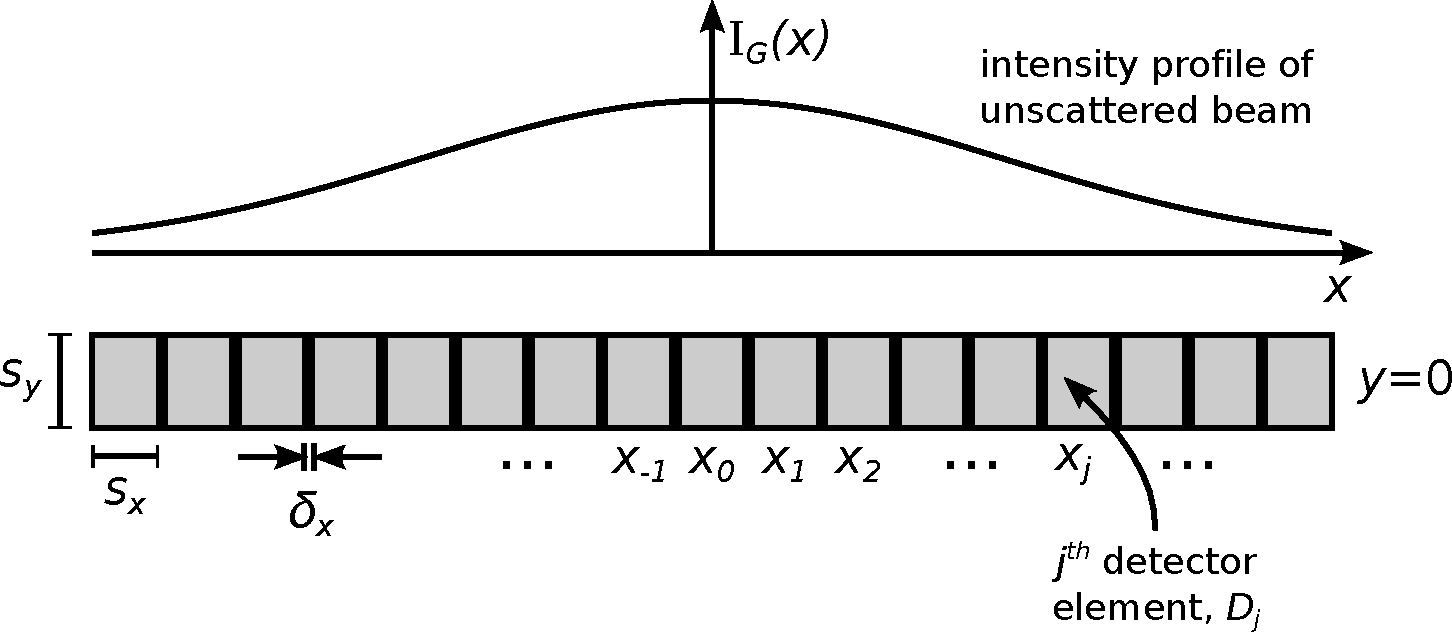
\includegraphics[width = \textwidth]{%
    Chapters/DesignConsiderations/figs/detector_array.pdf}
  \caption[Finite sampling-volume effects in a detector array]{%
    The probe radiation and the reference beam
    are interfered on a detector array.
    The array consists of numerous detector elements,
    each of size $s_x \times s_y$ and with interelement spacing $\delta_x$.
    The unscattered beam is centered on $x_0 = 0$ and $y = 0$, and
    its intensity profile varies only weakly over any given element.
    The finite size of each detector element tends to attenuate
    short wavelength components of the incident optical signal.
  }
\label{fig:DesignConsiderations:detector_array}
\end{figure}


\subsection{Spatial-structure mismatch between beams}
The external reference-beam interferometry derivations
in Section~\ref{sec:InterferometricMethods:interferometry}
assumed that the reference beam was exactly matched
in both amplitude and spatial structure
to the unscattered probe beam.
This is obviously an idealization
that, at best, can only be approached asymptotically in experiment.
This section discusses the geometric effects
of such imperfections in beam matching.

The derivation of the heterodyne intensity
(\ref{eq:InterferometricMethods:heterodyne_intensity})
can be easily generalized to account for
the geometric effects of unmatched reference and probe beams.
Namely, let the image-plane probe radiation be given by
\begin{equation}
  E_P(\vect{r}_{\image}, t)
  \approx
  E_{G,P}(\vect{r}_{\image}, t)
  e^{i \bar{\phi}}
  \left[%
    1
    +
    i \tilde{\phi}_0 \cos\nu
  \right],
\end{equation}
and let the corresponding reference beam be given by
\begin{equation}
  E_R(\vect{r}_{R}, t)
  =
  E_{G,R}(\vect{r}_{R}, t) e^{-i \Delta\omega_0 t},
\end{equation}
where $\vect{r}_{\image} = (x_{\image}, y_{\image}, z_{\image})$,
\begin{equation}
  \vect{r}_{R}
  =
  \vect{r}_{\image}
  +
  (0, 0, z_{R} - z_{\image}),
\end{equation}
and $E_{G,j}$ is a Gaussian beam
with angular frequency $\omega_0$,
waist amplitude $E_{0,j}$, and
waist 1/e $E$ radius $w_{0,j}$.
If $z_R \neq z_{\image}$,
the reference beam's waist sits at a different location
than that of the unscattered probe beam.
Under these circumstances, the heterodyne intensity becomes
\begin{equation}
  \begin{aligned}
    I_{\text{het}}(\vect{r}_{\image}, z_R, t)
    =
    2 I_{G,P}(\vect{r}_{\image})
    \bigl[%
      &\alpha_{\text{DC}}
      +
      \alpha_{\text{AC}}
      \cos(\Delta \omega_0 t + \bar{\phi}_{\text{eff}})
      \\
      &-
      \tilde{\phi}_0 \alpha_{\text{AC}}
      \sin(\Delta \omega_0 t + \bar{\phi}_{\text{eff}}) \cos\nu
    \bigr],
  \end{aligned}
  \label{eq:DesignConsiderations:heterodyne_intensity}
\end{equation}
where
\begin{equation}
  \bar{\phi}_{\text{eff}}
  =
  \bar{\phi}
  +
  \bigl[ \phi_{G,P}(\vect{r}_{\image}) - \phi_{G,R}(\vect{r}_R) \bigr]
\end{equation}
is the effective bulk phase,
\begin{equation}
  \phi_{G,j}(\vect{r})
  =
  k_0 z + \frac{k_0 \rho^2}{2 R_j(z)} - \psi_j(z)
\end{equation}
is the phase of Gaussian beam $j \in \{P, R\}$
(i.e.\ $E_{G,j}(\vect{r}) = |E_{G,j}(\vect{r})| e^{i \phi_{G,j}(\vect{r})}$),
\begin{align}
  \alpha_{\text{DC}}
  &=
  \frac{1}{2}\left[%
    1
    +
    \frac{I_{G,R}(\vect{r}_R)}{I_{G,P}(\vect{r}_{\image})}
  \right],
  \\
  \alpha_{\text{AC}}
  &=
  \sqrt{\frac{I_{G,R}(\vect{r}_R)}{I_{G,P}(\vect{r}_{\image})}},
\end{align}
are geometric factors that describe the amplitudes
of the DC and AC components of the heterodyne signal, and
\begin{equation}
  I_{G,j}(\vect{r})
  =
  \frac{c \varepsilon_0 |E_{G,j}(\vect{r})|^2}{2}
\end{equation}
is the intensity profile (averaged over an optical cycle)
of Gaussian beam $j \in \{P, R\}$.
Note that (\ref{eq:DesignConsiderations:heterodyne_intensity}) readily reduces to
(\ref{eq:InterferometricMethods:heterodyne_intensity})
if $E_{G,R}(\vect{r}_R) = E_{G,P}(\vect{r}_{\image})$.

It is worth discussing the implications of heterodyne intensity
(\ref{eq:DesignConsiderations:heterodyne_intensity}).
First, the AC component of the intensity
carries the desired phase information, and
maximizing the ratio of the AC signal to the DC signal requires that
$I_{G,R}(\vect{r}_R) = I_{G,P}(\vect{r}_{\image})$.
Second, note that the effective bulk phase $\bar{\phi}_{\text{eff}}$
is dependent on the geometry of the reference beam and
the unscattered probe beam.
Specifically, in the context of measuring
the plasma-induced bulk phase $\bar{\phi}$,
note that
\begin{equation}
  \bar{\phi}_{\text{eff}}(\rho_{\image}=0)
  =
  \bar{\phi}
  +
  k_0 (z_{\image} - z_R)
  -
  \left[ \psi_P(z_{\image}) - \psi_R(z_R) \right].
\end{equation}
If $z_{\image}$ and $z_R$ are fixed,
then the beam-geometry contributions to
$\bar{\phi}_{\text{eff}}(\rho_{\image} = 0)$
constitute an unimportant DC offset that can be removed
via baseline subtraction;
however, experiments are typically plagued by vibrations, and
even small changes to $z_{\image}$ and $z_R$
can make significant time-dependent contributions to
$\bar{\phi}_{\text{eff}}(\rho_{\image} = 0)$ at CO$_2$ probe wavelengths.
As such, deconvolving the plasma-induced and vibration-induced contributions
to $\bar{\phi}_{\text{eff}}(\rho_{\image} = 0)$
requires interferometric measurements
at two distinct wavelengths (i.e.\ two-color interferometry)
\cite{carlstrom_rsi88}.
However, such vibrations occur on slow time-scales
(e.g.\ $f_{\text{vib}} \lesssim \SI{5}{\kilo \hertz}$),
and phase measurements at a \emph{single} wavelength are sufficient
to quantify plasma-induced phase fluctuations
at frequencies above $f_{\text{vib}}$
\cite{vanzeeland_ppcf05}.
Note that the beam geometry also imparts
a spatially dependent, curvature-induced phase shift
\begin{align}
  \delta\phi_{\kappa}(\rho_{\image})
  &=
  \bar{\phi}_{\text{eff}}(\rho_{\image})
  -
  \bar{\phi}_{\text{eff}}(\rho_{\image} = 0)
  \notag \\
  &=
  \frac{k_0 \rho_{\image}^2}{2}
  \left[\frac{1}{R_P(z_{\image})} - \frac{1}{R_R(z_R)} \right],
\end{align}
which can result in signal loss and distortion of the measured wavenumber.
To see this, assume that the radiation is interfered on a detector array,
as shown in Fig.~\ref{fig:DesignConsiderations:detector_array}.
As a detector element produces a signal
proportional to the average intensity across its face,
there will be substantial signal loss
if there are large curvature-induced phase shifts
across the element's face
(i.e.\ $\delta\phi_{\kappa}(s_x / 2) \gtrsim \pi$ or
$\delta\phi_{\kappa}(s_y / 2) \gtrsim \pi$).
Further, if there are large curvature-induced phase shifts
across the length of the detector array,
the spatial structure of the intensity
will \emph{not} correspond to the spatial structure
of the plasma fluctuation.
The latter is the more conservative constraint
on the curvature-induced phase shift.
Assuming that the detector array shown in
Fig.~\ref{fig:DesignConsiderations:detector_array}
consists of $N_{\text{el}}$ detector elements and
that the inter-element spacing is negligible ($\delta_x \ll s_x$),
the criterion for negligible curvature-induced phase shifts
$\delta\phi_{\kappa, \text{max}}
=
\delta\phi_{\kappa}(\rho_{\image, \text{max}})
\ll
1$
becomes
\begin{equation}
  \frac{k_0}{8}
  \left[ (N_{\text{el}} s_x)^2 + s_y^2 \right]
  \left| \frac{1}{R_P(z_{\image})} - \frac{1}{R_R(z_R)}\right|
  \ll
  \pi.
\end{equation}


\section{Phase noise: sources and effects}


\subsection{Umatched optical path lengths}
The external reference-beam interferometry derivations
in Section~\ref{sec:InterferometricMethods:interferometry}
assumed that the laser's angular frequency was fixed
at its nominal value $\omega_0$.
However, the angular frequency of any \emph{real} laser
will exhibit short-term jitter and long-term drift,
much like any other real-world oscillator
\cite[Sec.~1.7]{siegman_lasers}.
The electric field of a Gaussian beam
with short-term frequency jitter
is well-described by
\begin{equation}
  E_G(\vect{r}, t)
  =
  E_G(\vect{r})
  e^{-i [\omega_0 t + \phi_{\omega_0}(t)]},
\end{equation}
where $\phi_{\omega_0}(t)$ is a zero-mean, stationary, random process
whose temporal variation causes
the oscillator's instantaneous angular frequency
to wander about its nominal value $\omega_0$.

Now, if the interferometer's probe beam and reference beam
traverse different optical path lengths,
the laser's short-term jitter will inject
phase noise into the measured signal.
To see this, assume that the optical path length of the probe beam
exceeds that of the reference arm by $L$.
Then, if the reference beam impinging on the detector at time $t$ is
\begin{equation}
  E_R(\vect{r}_{\image}, t)
  =
  E_G(\vect{r}_{\image})
  e^{-i [
    (\omega_0 + \Delta \omega_0) t
    +
    \phi_{\omega_0}(t)
  ]},
\end{equation}
the corresponding imaged probe radiation is
\begin{equation}
  E_P(\vect{r}_{\image}, t)
  =
  E_G(\vect{r}_{\image})
  e^{-i [\omega_0 (t - \tau) + \phi_{\omega_0}(t - \tau)]}
  e^{i \bar{\phi}}
  \left[%
    1
    +
    i \tilde{\phi}_0 \cos\nu
  \right],
\end{equation}
where $\tau = L / c$ is the time delay
associated with the optical path-length difference $L$.
Define the jitter-induced phase difference
\begin{equation}
  \delta \phi_{\omega_0}(t, \tau)
  =
  \phi_{\omega_0}(t + \tau)
  -
  \phi_{\omega_0}(t).
\end{equation}
Typically, $\delta \phi_{\omega_0}(t, \tau) \ll 1$.
Then, appropriately generalizing the derivations between
(\ref{eq:InterferometricMethods:heterodyne_intensity}) and
(\ref{eq:InterferometricMethods:heterodyne_total_fluctuating_intensity}),
one readily finds that the total fluctuating power
in the heterodyne interferometer's demodulated signals is
\begin{equation}
  \tilde{I}_{IQ}(\vect{r}_{\image}, t)
  =
  I_G(\vect{r}_{\image})
  \left[%
    \tilde{\phi}(x_{\image}, t)
    +
    \delta \phi_{\omega_0}(t - \tau, \tau)
  \right],
\end{equation}
and the measured phase fluctuation
$\tilde{\phi}_{\text{meas}}(x_{\image}, t)
=
\tilde{I}_{IQ}(\vect{r}_{\image}, t) / I_G(\vect{r_{\image}})$ is
\begin{equation}
  \tilde{\phi}_{\text{meas}}(x_{\image}, t)
  =
  \tilde{\phi}(x_{\image}, t)
  +
  \delta \phi_{\omega_0}(t - \tau, \tau);
  \label{eq:DesignConsiderations:measured_phase_with_laser_jitter}
\end{equation}
that is, the fluctuating signal is contaminated
by the laser's jitter.

\graffito{\textcolor{red}{Consistent notation and units with Appendix??}}
\textcolor{red}{%
  The phase noise of an oscillator is discussed in
  Appendix~\ref{app:OscillatorPhaseNoise}.
  Whereas the phase noise $\delta \phi_{\omega_0}(t - \tau, \tau)$
  is a complicated function of the externally imposed time delay $\tau$,
  the phase noise's autospectral density $S_{\delta \phi_{\omega_0}}(f)$
  can be explicitly related to the autospectral density of
  the laser's underlying frequency deviation $S_{\delta \nu_0}(f)$ via
  % (\ref{eq:OscillatorPhaseNoise:phase_noise_autospectral_density}),
  which is repeated here for completeness:
  \begin{equation}
    S_{\delta \phi_{\omega_0}}(f)
    =
    [2 \pi \tau \sinc(f \tau)]^2 S_{\delta \nu_0}(f).
  \end{equation}
  Thus, the autospectral density of the measured phase fluctuation from
  (\ref{eq:DesignConsiderations:measured_phase_with_laser_jitter})
  becomes
  \graffito{\textcolor{red}{Note about cancellation of uncorrelated cross terms}}
  \begin{equation}
    S_{\tilde{\phi}_{\text{meas}}}(f)
    =
    S_{\tilde{\phi}}(f)
    +
    [2 \pi \tau \sinc(f \tau)]^2 S_{\delta \nu_0}(f)
  \end{equation}
  Thus, the error in the autospectral density of the measured phase
  is linearly related to the autospectral density
  of the laser's underlying frequency deviation and
  quadratically related to the time delay $\tau$.
}


\subsection{Modulator's finite coupling time}
Heterodyne detection is effected by
modestly Doppler shifting the reference beam
relative to the plasma beam.
It is easy to Doppler shift $\SI{10.6}{\micro\meter}$ radiation
by tens of $MHz$ with a Germanium acousto-optic modulator (AOM).
The operation of a typical AOM is sketched in
Fig.~\ref{fig:DesignConsiderations:aom_scattering_diagram}.
A piezo-actuator drives sound waves
of angular frequency $\Delta \omega_0$
through the Germanium crystal, and
the sound waves act as a diffraction grating
that propagates at the crystal's sound speed $c_s$.
When a beam of vacuum wavelength $\lambda_0$
impinges upon the crystal at the Bragg angle
\graffito{\textcolor{red}{comment about Bragg regime criterion from Ch.~2?}}
\begin{equation}
  \theta_B = \frac{\lambda_0 \cdot \Delta \omega_0}{4 \pi c_s},
  \label{eq:DesignConsiderations:Bragg_angle}
\end{equation}
a portion of the beam is deflected and
Doppler shifted by angular frequency $\Delta \omega_0$
\cite[Sec.~20.1]{saleh_and_teich}.
The power in the deflected beam
is controlled by the intensity of the sound waves.

\begin{figure}
  \centering
  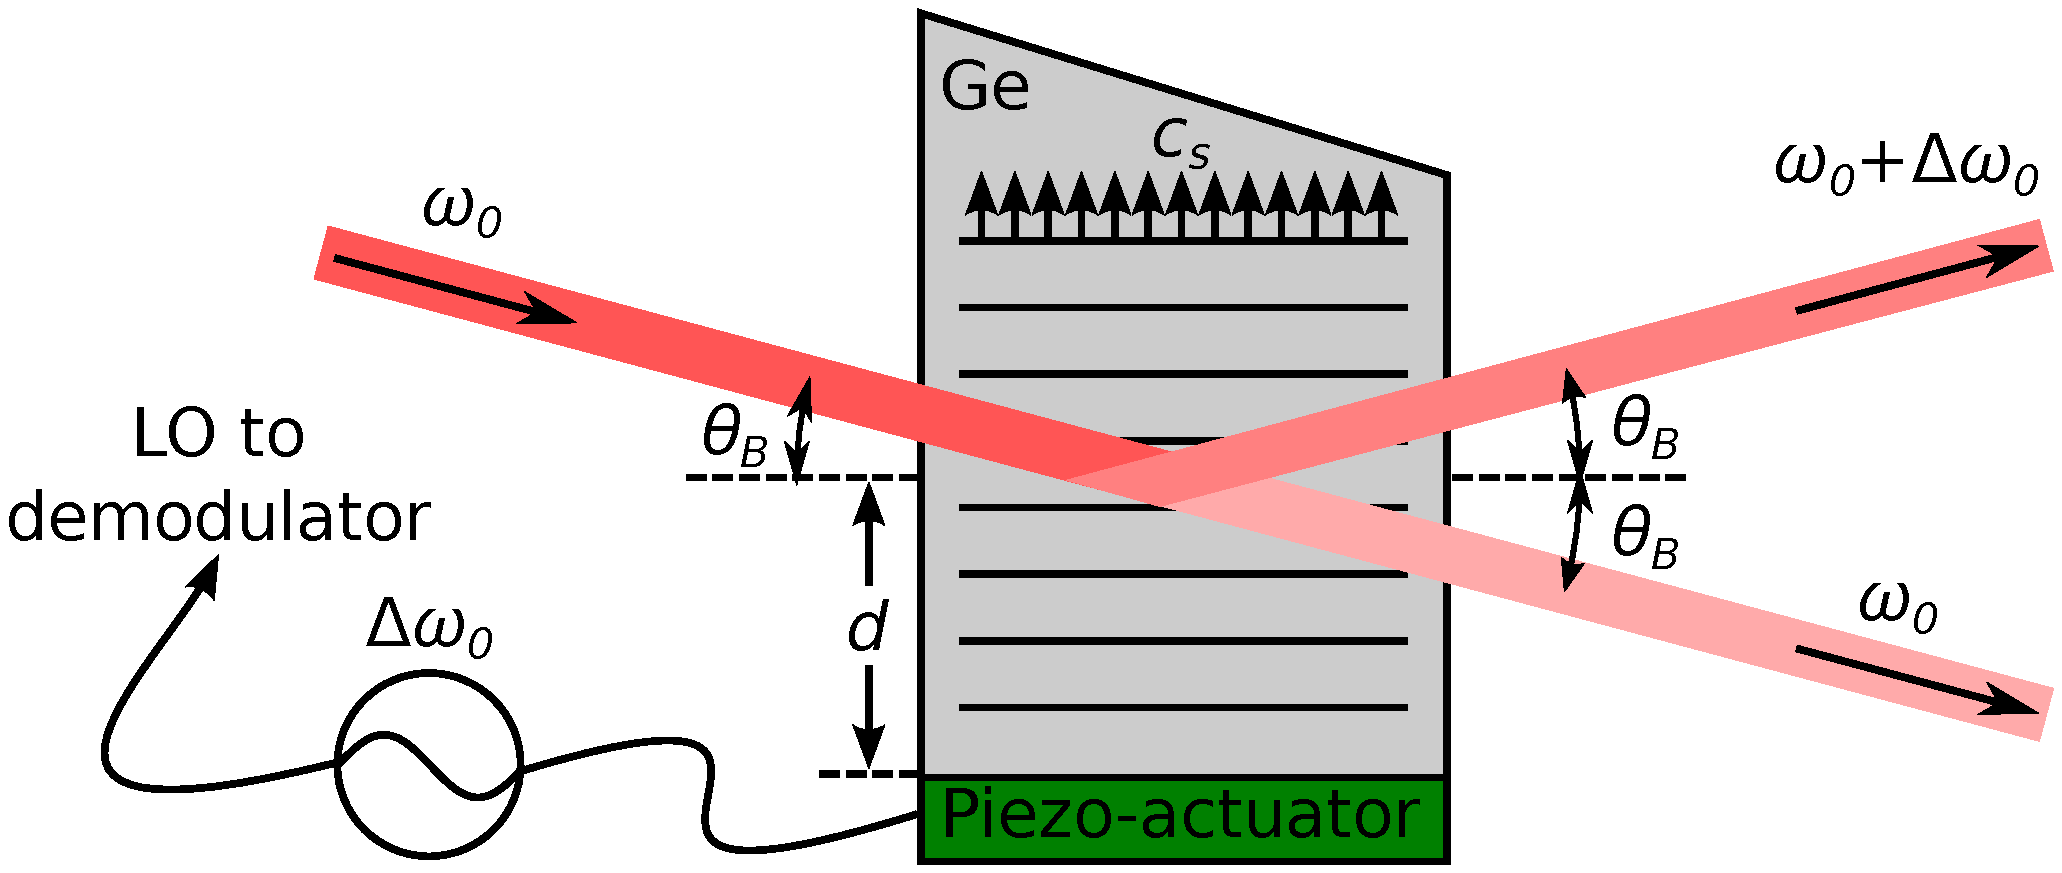
\includegraphics[width = \textwidth]{%
    Chapters/DesignConsiderations/figs/aom_scattering_diagram.pdf}
  \caption[Illustration of AOM operation in a heterodyne interferometer]{%
    An illustration of AOM operation in a heterodyne interferometer.
    A piezo-actuator drives sound waves of angular frequency $\Delta \omega_0$
    through a crystal (usually Germanium for $\SI{10.6}{\micro\meter}$ light),
    and these sound waves deflect and Doppler shift light
    that is incident upon the crystal at the Bragg angle $\theta_B$.
    The sound waves propagate from the piezo-actuator
    to the AOM's optically active region
    over finite time $\tau = d / c_s$.
    The RF waveform that drives the piezo-actuator
    is sampled and used to demodulate the heterodyne interference signal.
    Note that for simplicity the refraction of the beam
    as it enters and exits the crystal is \emph{not} depicted.}
\label{fig:DesignConsiderations:aom_scattering_diagram}
\end{figure}

The coupling of the AOM's drive signal to the deflected beam
occurs on the crystal's sound-wave timescale.
If the sound waves must propagate a distance $d$
from the piezo-actuator to the AOM's optically active region,
the drive signal is coupled to the deflected beam
only after time delay $\tau = d / c_s$.
\graffito{\textcolor{red}{reference?}}
The sound speed in Germanium is $c_s = \SI{5400}{\meter\per\second}$
such that a distance $d = \SI{1}{\centi\meter}$
is accompanied by a time delay $\tau = \SI{1.85}{\micro\second}$.
Note that this is large compared to many other timescales
typically considered in interferometry;
for example, light propagates
through $\SI{1}{\meter}$ of air
in only $\SI{3.33}{\nano\second}$,
and an RF signal propagates
through $\SI{1}{\meter}$ of RG-58 coaxial cable
(for which the index of refraction is $\sim 3 / 2$)
in only $\SI{5}{\nano\second}$.

In the presence of local-oscillator jitter,
an AOM's finite coupling time
can degrade the performance of a heterodyne interferometer.
A local oscillator with short-term jitter is well-described by
\begin{equation}
  V_{\text{LO}}(t)
  =
  V_{0}
  e^{-i [\Delta \omega_0 t + \phi_{\Delta \omega_0}(t)]},
\end{equation}
where $\phi_{\Delta \omega_0}(t)$ is a zero-mean, stationary, random process
whose temporal variation causes
the local oscillator's instantaneous angular frequency
to wander about its nominal value $\Delta \omega_0$.
As discussed in the previous paragraph,
the AOM's finite coupling time far exceeds
the few tens of nanoseconds required for the beam
to propagate through an interferometer
of optical path length $\sim \SI{10}{\meter}$.
Thus, to account for the AOM's finite coupling time and
the local oscillator's jitter, take
$\Delta \omega_0 t
\rightarrow
[\Delta \omega_0 (t - \tau) + \phi_{\Delta \omega_0}(t - \tau)]$
in the heterodyne intensity
(\ref{eq:InterferometricMethods:heterodyne_intensity}).
Then, assuming negligible finite sampling-volume effects,
the heterodyne output voltage
from a detector element at position $\vect{r}_{\image}$
is simply proportional to the local intensity intensity, i.e.\
\begin{align}
  \begin{aligned}
    V_{\text{het}}(\vect{r}_{\image}, t)
    &=
    2 V_0
    \bigl\{%
      1
      +
      \cos\left[%
        \Delta \omega_0 t
        +
        \bar{\phi}_{\text{eff}}
        +
        \phi_{\Delta \omega_0}(t - \tau)
      \right]
      \\
      &\quad-
      \tilde{\phi}(x_{\image}, t)
      \sin\left[%
        \Delta \omega_0 t
        +
        \bar{\phi}_{\text{eff}}
        +
        \phi_{\Delta \omega_0}(t - \tau)
      \right]
    \bigr\},
  \end{aligned}
\end{align}
where $\bar{\phi}_{\text{eff}} = \bar{\phi} - \Delta \omega_0 \tau$.
Then, following the same demodulation ``program'' used between
(\ref{eq:InterferometricMethods:heterodyne_interferometer_I_and_Q_intensity})
and
(\ref{eq:InterferometricMethods:heterodyne_total_fluctuating_intensity}),
the demodulated in-phase ($V_I$) and quadrature ($V_Q$) signals are defined as
\graffito{\textcolor{red}{Sign \& arg.\ of $\delta \phi_{\Delta \omega_0}$??}}
\begin{align}
  V_{I}(t)
  +
  i \cdot V_{Q}(t)
  &=
  \frac{1}{V_0}
  \langle
    V_{\text{LO}}(t)
    \cdot
    V_{\text{het}}(t)
  \rangle_{\Delta \omega_0}
  \notag \\
  &=
  V_0
  e^{i \bar{\phi}_{\text{eff}}}
  \left[
    \tilde{\phi}(x_{\image}, t)
    +
    \delta \phi_{\Delta \omega_0}(t - \tau, \tau)
  \right],
\end{align}
and the total fluctuating voltage in the demodulated signals is
\begin{equation}
  \tilde{V}_{IQ}(t)
  =
  V_0
  \left[
    \tilde{\phi}(x_{\image}, t)
    +
    \delta \phi_{\Delta \omega_0}(t - \tau, \tau)
  \right].
\end{equation}
Thus, the measured phase fluctuation
$\tilde{\phi}_{\text{meas}}(x_{\image}, t)
=
\tilde{V}_{IQ}(t) / V_0$
becomes
\graffito{\textcolor{red}{Sign \& arg.\ of $\delta \phi_{\Delta \omega_0}$??}}
\begin{equation}
  \tilde{\phi}_{\text{meas}}(x_{\image}, t)
  =
  \tilde{\phi}(x_{\image}, t)
  +
  \delta \phi_{\Delta \omega_0}(t - \tau, \tau);
\end{equation}
that is, the fluctuating signal is contaminated
by the local oscillator's jitter.

\begin{itemize}
  \item \textcolor{red}{modify corresponding path-length matching as needed}
\end{itemize}


\section{Amplitude noise: sources and effects}
Detector noise and shot noise are typically
the largest contributors to amplitude noise
in the heterodyne interference signal, while
a noisy amplifier can degrade the signal-to-noise ratio.
The demodulation of such amplitude noise
is throughly discussed by Rakhmanov in~\cite{rakhmanov_ao01}.
While Rakhmanov does not explicitly consider quadrature heterodyne detection,
his results can be naturally applied to quadrature heterodyne detection,
as is done below.


\subsection{Detector noise}
\graffito{\textcolor{red}{check signs and write more clearly}}
Real-world detector operation is associated with intrinsic noise.
This noise results from, among other things,
Johnson thermal noise in the detector and its associated electronics
and shot noise in the background radiation flux
\cite{hamamatsu_ir_detectors}.
A detector's noise is often characterized by
its noise-equivalent power ($NEP$):
when the power of the incident optical signal is equal to the $NEP$,
the signal-to-noise ratio is unity.
For a measurement with temporal bandwidth $\Delta f$,
a detector element with effective area $A$
will have an $NEP$
\begin{equation}
  NEP = \frac{\sqrt{A \cdot \Delta f}}{D^{*}},
\end{equation}
where $D^{*}$ is the detector's specific detectivity
\cite{jones_josa60}.
Note that larger $D^{*}$ corresponds to increased detector sensitivity.

Signal demodulation pushes detector noise
near the heterodyne frequency $\Delta \omega_0$
into the baseband signal, as is now demonstrated.
Note that
\begin{equation}
  NEP = \left\{ E\left[ \left| \delta P(t) \right|^2 \right] \right\}^{1/2},
\end{equation}
where $\delta P(t)$ is a real-valued, zero-mean, stationary, random process
that gives rise to the $NEP$ and
$E$ is the expectation-value operator.
Following a formalism similar to that from
Section~\ref{sec:InterferometricMethods:interferometry:heterodyne},
the detector noise in the in-phase ($I$) channel will be
\begin{equation}
  \delta P_I(t)
  =
  \left.
    \left[
      \cos(\Delta \omega_0 t) \cdot \delta P(t)
    \right]
  \right|_{|\omega| \ll \Delta \omega_0},
\end{equation}
and the detector noise in the quadrature ($Q$) channel will be
\begin{equation}
  \delta P_Q(t)
  =
  \left.
    \left[
      \sin(\Delta \omega_0 t) \cdot \delta P(t)
    \right]
  \right|_{|\omega| \ll \Delta \omega_0}.
\end{equation}
These two powers can be conveniently combined as
\begin{align}
  \delta P_{IQ}(t)
  &=
  \delta P_{I}(t) - i \cdot \delta P_{Q}(t)
  \notag \\
  &=
  \left.
    \left[
      e^{- i \Delta \omega_0 t} \cdot \delta P(t)
    \right]
  \right|_{|\omega| \ll \Delta \omega_0}.
\end{align}
Then, the autocorrelation function of corresponding baseband noise is
\begin{align}
  R_{\delta P_{IQ},\delta P_{IQ}}(\tau)
  &=
  E\left[\delta P_{IQ}(t) \cdot \delta P_{IQ}(t + \tau) \right]
  \notag \\
  &=
  e^{i \Delta \omega_0 \tau} \cdot R_{\delta P, \delta P}(\tau),
\end{align}
where $R_{\delta P, \delta P}(\tau)$ is the
autocorrelation function of the detector noise.
The corresponding autospectral density
of the demodulated detector noise is then
\begin{align}
  S_{\delta P_{IQ},\delta P_{IQ}}(\omega)
  &=
  \mathcal{F}\left[ R_{\delta P_{IQ},\delta P_{IQ}}(\tau) \right](\omega)
  \notag \\
  &=
  \mathcal{F}\left[
    e^{i \Delta \omega_0 \tau} \cdot R_{\delta P, \delta P}(\tau)
  \right](\omega)
  \notag \\
  &=
  S_{\delta P, \delta P}(\omega - \Delta \omega_0)
  \notag \\
  &\approx
  S_{\delta P, \delta P}(\Delta \omega_0),
  \label{eq:DesignConsiderations:detector_noise_demodulated}
\end{align}
\graffito{\textcolor{red}{$\sim \SI{e-18}{\watt\squared\per\hertz}$}}
where $S_{\delta P, \delta P}$ is
the autospectral density of the detector noise, and
the approximation follows from
the low-pass filtering
(i.e.\ $|\omega| \ll \Delta \omega_0$) and
the realness of $\delta P$
(i.e.\ $S_{\delta P, \delta P}(-\omega) = S_{\delta P, \delta P}(\omega)$).
That is, the detector noise at the heterodyne frequency $\Delta \omega_0$
is pushed into the baseband signal via the demodulation process.
Note that the autospectral density of the demodulated detector noise
(\ref{eq:DesignConsiderations:detector_noise_demodulated})
is in agreement with the literature
(e.g.\ see Rakhmanov's Eq.~(47) in~\cite{rakhmanov_ao01}
with $d_1 = 1 / 2$ for demodulation against a perfect sinusoid;
whereas Rakhmanov considers only \emph{one} of the demodulated channels,
(\ref{eq:DesignConsiderations:detector_noise_demodulated})
considers both the in-phase and quadrature channels and
is thus twice as large as Rakhmanov's expression).


\subsection{Shot noise}
The discrete nature of the arriving photons results in shot noise.
Well-modeled as a Poisson process,
the shot noise increases as $N_{\gamma}^{1/2}$, where
$N_{\gamma}$ is the number of incident photons.
Because the incident optical power (and hence the number of incident photons)
in the heterodyne optical signal is modulated as a function of time,
the corresponding shot noise is inherently \emph{nonstationary}.
Surprisingly, however, the demodulated shot noise \emph{is} stationary
(e.g.\ see Rakhmanov's Eq.~(59) in~\cite{rakhmanov_ao01}).
Note that Rakhmanov only considers \emph{one} of the demodulated signals, and
maximizing the signal-to-noise ratio in the demodulated signal
requires careful selection of the local oscillator's phase
relative to that of the heterodyne signal
(he terms this the ``demodulation phase'' and
represents it via $\gamma$).
However, by employing quadrature heterodyne detection~\cite{carlstrom_rsi88},
in which $\gamma_Q = \gamma_I + \pi / 2$,
the dependence on the demodulation phase vanishes; that is
\graffito{\textcolor{red}{$\sim \SI{e-21}{\watt\squared\per\hertz}$}}
\begin{align}
  S_{\delta P_{IQ}, \delta P_{IQ}}(\omega)
  &=
  S_{\delta P_{I}, \delta P_{I}}(\omega; \gamma_I)
  +
  S_{\delta P_{Q}, \delta P_{Q}}(\omega; \gamma_Q)
  \notag \\
  &=
  \hbar \omega_0 P_0,
\end{align}
where $\hbar$ is the Planck constant divided by $2 \pi$,
$\omega_0$ is the angular frequency of the incident photons, and
$P_0$ is the DC optical power impinging upon the detector.


\subsection{Amplifier noise}
The noise \emph{factor} $F$ of an RF amplifier is defined as the ratio of
the signal-to-noise ratio at the device's input ($SNR_{\text{in}}$) to
the signal-to-noise ratio at the device's output ($SNR_{\text{out}}$)
\begin{equation}
  F = \frac{SNR_{\text{in}}}{SNR_{\text{out}}};
\end{equation}
often, the noise factor $F$ is given
in terms of the noise \emph{figure} $NF$
\cite{minicircuits_amplifier_terms_defined}
\begin{equation}
  NF = 10 \log_{10} F.
\end{equation}
If several amplifiers are cascaded,
the total noise factor of the amplifier chain
can be computed using the well-known Friis noise-factor formula.
Note that the noise factor is only defined
in the context of a signal-to-noise ratio, so
it is not possible to write down the corresponding
autospectral density of the amplifier noise in absolute units.


\section{Quantization noise}
Efficient conversion of an analog signal to a digital record requires
quantization of the signal magnitude and
temporal sampling of these quantized magnitudes~\cite{bennett_bstj48}.
This analog-to-digital conversion
is performed by an instrument known as a digitizer.
If a digitizer has bit depth $N_b$ and
an input-voltage dynamic range $V_{\text{dyn}}$,
then its quantum of voltage $\Delta V$ is
\begin{equation}
  \Delta V
  =
  \frac{V_{\text{dyn}}}{2^{N_b} - 1}
  \approx
  \frac{V_{\text{dyn}}}{2^{N_b}},
  \label{eq:DesignConsiderations:digitizer_voltage_quantum}
\end{equation}
where the approximation is well-satisfied
for typical digitizer bit depths.
At each sampling time,
the analog signal's magnitude is approximated
by the closest quantized value, whose
separation from the true, analog value
will be less than or equal to $\Delta V / 2$.

In general, then, the quantized signal
will differ from the analog signal.
This error $\epsilon$ is known as quantization noise.
The mean square error (i.e.\ variance) attributable to quantization is simply
\begin{equation}
  \overline{\epsilon^2} = \frac{(\Delta V)^2}{12},
  \label{eq:DesignConsiderations:quantization_noise_variance}
\end{equation}
where $\Delta V$ is the digitizer's quantum of voltage,
as given by (\ref{eq:DesignConsiderations:digitizer_voltage_quantum})
\cite{bennett_bstj48}
\cite[Sec.~10.2.4]{bendat_and_piersol}.
For a uniformly sampled record with sampling rate $f_s$,
sufficiently fine quantization $\Delta V$
ensures that the quantization noise is \emph{white}
\cite[Th.~1]{bennett_bstj48}
\cite[Ch.~20]{widrow_and_kollar};
that is, the autospectral density of the quantization noise is
\begin{align}
  S_{\epsilon,\epsilon}(f)
  =
  \frac{\overline{\epsilon^2}}{f_s}
  =
  \frac{(\Delta V)^2}{12 f_s},
  \qquad
  -f_s < f \leq f_s.
  \label{eq:DesignConsiderations:quantization_noise_autospectral_density}
\end{align}
In practice, however, aperture error, jitter, and nonlinearities
may reduce the effective bit depth by one or two bits
\cite[Sec.~10.2.4]{bendat_and_piersol},
increasing the realized quantization noise
relative to that expected from
(\ref{eq:DesignConsiderations:quantization_noise_variance}) and
(\ref{eq:DesignConsiderations:quantization_noise_autospectral_density}).

Quantization noise can be significant
when attempting to measure absolute phase fluctuations
with a heterodyne interferometer.
Recall from the discussion of heterodyne interferometric detection in
Section~\ref{sec:InterferometricMethods:interferometry:heterodyne}
that measurement of the \emph{absolute} phase
requires capturing the full dynamics
of the large, slowly varying equilibrium phase $\bar{\phi}$
in addition to measurement of the fluctuating phase $\tilde{\phi}$.
Because $\tilde{\phi} \ll \bar{\phi}$ in typical situations,
the fluctuations only occupy a small portion
of the digitizer's dynamic range; that is,
fluctuations effectively see a bit depth that
is substantially smaller than the digitizer's nominal bit depth.
Thus, to minimize the effect of quantization noise,
it is absolutely imperative
to utilize the full dynamic range of the digitizer.


\section{Demodulation}
\begin{itemize}
  \item Focus below is on analog, rather than digital, demodulation
\end{itemize}


\subsection{Ideal demodulation}
\label{sec:DesignConsiderations:demodulation:ideal}
A typical analog $I\&Q$ demodulator consists of
a $90^{\circ}$ splitter,
two double-balanced mixers, and
a $0^{\circ}$ splitter~\cite{minicircuits_modulators}, as shown in
Fig.~\ref{fig:DesignConsiderations:analog_IQ_demodulator}(a).
The $90^{\circ}$ splitter divides the incident local oscillator (LO) signal
\begin{equation}
  \text{LO}(t) = \cos(\Delta\omega_0 t)
\end{equation}
into an ``in-phase'' copy of the LO
\begin{equation}
  \text{LO}_0(t)
  =
  \frac{1}{\sqrt{2}} \cos(\Delta\omega_0 t)
\end{equation}
and a $\pi / 2$-phase-advanced copy of the LO
\begin{equation}
  \text{LO}_{\pi / 2}(t)
  =
  \frac{1}{\sqrt{2}} \cos\left( \Delta\omega_0 t + \frac{\pi}{2} \right)
  =
  - \frac{1}{\sqrt{2}} \sin(\Delta\omega_0).
\end{equation}
Note that the power in the incident LO signal
is split evenly between $\text{LO}_0(t)$ and $\text{LO}_{\pi / 2}(t)$.
The $0^{\circ}$ splitter divides the intermediate frequency (IF) signal
\begin{equation}
  \text{IF}(t) = A_{\text{IF}} \cos(\Delta\omega_0 t + \phi)
  \label{eq:DesignConsiderations:IF_perfect_sinusoid}
\end{equation}
into two nominally identical copies of the IF
\begin{equation}
  \text{IF}_0(t)
  =
  \frac{A_{\text{IF}}}{\sqrt{2}} \cos(\Delta\omega_0 t + \phi).
\end{equation}
Like the LO signal, the power in the incident IF signal
is split evenly between the two copies.
The signal at the demodulator's in-phase ($I$) port
then corresponds to the product of
$\text{IF}_0(t)$ with the in-phase LO signal $\text{LO}_0(t)$:
\graffito{\textcolor{red}{incorrect amplitude}}
\begin{equation}
  \text{LO}_0(t) \cdot \text{IF}_0(t)
  =
  \frac{A_{\text{IF}}}{\sqrt{2}}
  \left[
    \cos(\phi) + \cos(2 \Delta\omega_0 t + \phi)
  \right].
\end{equation}
Such signal multiplication is often referred to as ``mixing''.
Low-pass filtering the signal exiting the demodulator's $I$ port
yields the baseband in-phase signal
\begin{equation}
  I = \frac{A_{\text{IF}}}{\sqrt{2}} \cos\phi.
\end{equation}
Similar reasoning regarding the product
$\text{LO}_{\pi / 2}(t) \cdot \text{IF}_0(t)$
at the demodulator's quadrature ($Q$) port
yields the baseband quadrature signal
\begin{equation}
  Q = \frac{A_{\text{IF}}}{\sqrt{2}} \sin\phi.
\end{equation}
Note that the total power in the $I\&Q$ signals
is $\SI{3}{\decibel}$ lower
than the power in the incident IF signal.
This is known as the \emph{conversion loss} of the demodulator, and
it results from low-pass filtering the $I\&Q$ signals;
real-world demodulators will have larger conversion losses
due to the additional effects of dissipation and other nonideal effects.
An \emph{absolute} phase measurement $\phi_m$ is then obtained via
\begin{equation}
  \phi_m = \atan\left( \frac{Q}{I} \right),
  \label{eq:DesignConsiderations:phase_from_arctangent}
\end{equation}
independent of the power in the incident IF signal.
Note that in the ideal case the measured phase is
equal to the true phase, i.e.\ $\phi_m = \phi$.

\begin{figure}
  \centering
  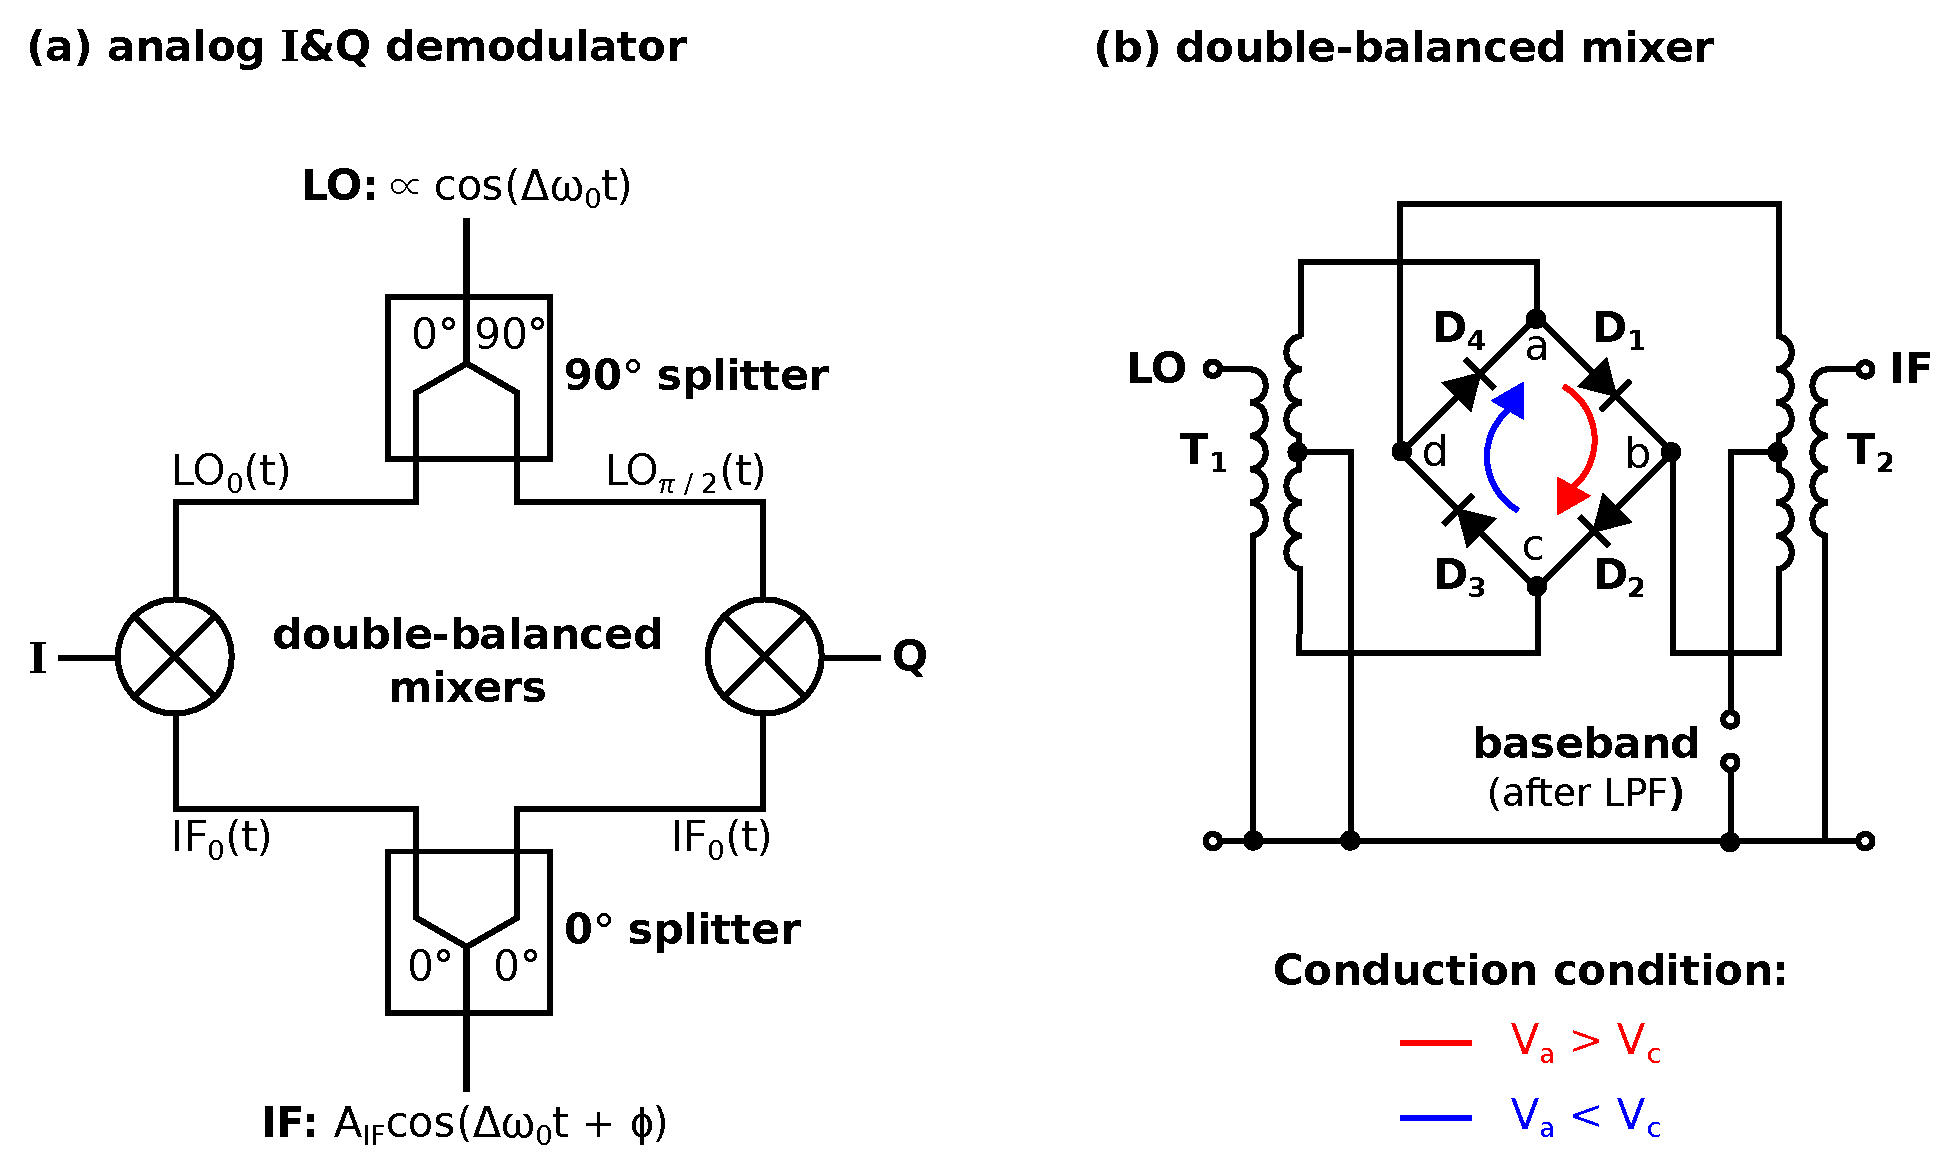
\includegraphics[width = \textwidth]{%
    Chapters/DesignConsiderations/figs/analog_IQ_demodulator.pdf}
  \caption[Components of a typical analog $I\&Q$ demodulator]{%
    (a) A typical analog $I\&Q$ demodulator and
    (b) a typical diode-ring double-balanced mixer.
    \textcolor{red}{Baseband??? More thorough descriptions}}
  \label{fig:DesignConsiderations:analog_IQ_demodulator}
\end{figure}


\subsection{Nonideal mixing}
\label{sec:DesignConsiderations:demodulation:nonideal_mixing}
In Section~\ref{sec:DesignConsiderations:demodulation:ideal},
mixing was idealized as the multiplication of the IF signal by the LO signal.
However, in practice, more complex process are used
to maximize the mixer's linear dynamic range and minimize its noise figure
\cite{analog_devices_mix_and_mod,bryant_mult_vs_mod}.

For example, a typical ring-diode double-balanced mixer
is shown in Fig.~\ref{fig:DesignConsiderations:analog_IQ_demodulator}(b).
The balun transformers $T_1$ and $T_2$
isolate the baseband port from the LO and IF ports.
Typically, the LO power is $\sim \SI{20}{\deci\bel}$ larger than the IF power.
As a result, the LO alone is responsible
for biasing the mixer's diodes into conduction.
Note that the diodes are not all simultaneously biased into conduction.
Instead, when $V_a > V_c$ (neglecting the diode drops),
diodes $D_1$ and $D_2$ are forced into conduction such that
$V_b$ acts as a virtual ground for the IF signal
coupled through transformer $T_2$.
Then, when the LO changes sign such that $V_a < V_c$,
diodes $D_1$ and $D_2$ stop conducting, and
diodes $D_3$ and $D_4$ begin to conduct,
forcing the virtual ground to jump from $V_b$ to $V_d$.
Thus, the ring diode acts as a switch
for the polarization of the coupled IF signal,
with the switching governed by the sign and frequency of the LO.
Low-pass filtering the polarization-modulated IF, of course,
yields the desired baseband signal.
Note that the diode switching time should be minimized
for optimal modulation,
explaining why some manufacturers
advocate the use of a square, rather than a sinusoidal, LO
\cite{minicircuits_mixer_faqs}.

\begin{figure}
  \centering
  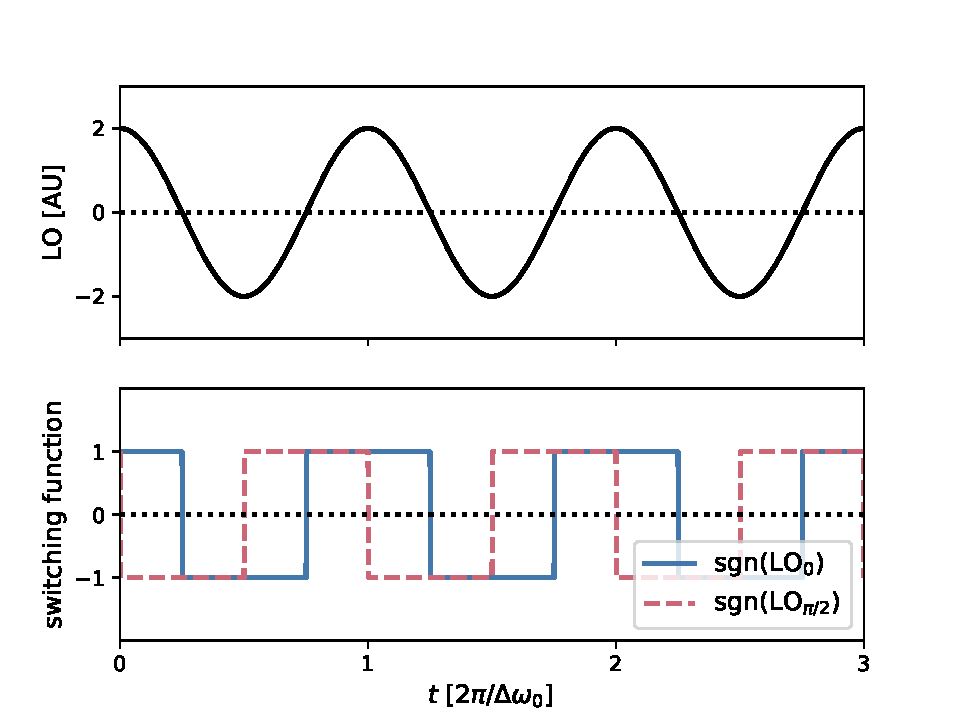
\includegraphics[width = \textwidth]{%
    Chapters/DesignConsiderations/figs/LO_switching_function.pdf}
  \caption[LO switching functions]{%
    The LO switching functions.
    The top panel displays the incident sinusoidal LO signal, while
    the bottom panel shows the \emph{sign} of
    the in-phase ($\text{LO}_0$) and
    the $\pi / 2$ phase-advanced ($\text{LO}_{\pi / 2}$)
    copies of the LO signals.}
  \label{fig:DesignConsiderations:LO_switching_function}
\end{figure}

This polarization modulation can alter the baseband spectrum.
To see this, note that the sign of the in-phase LO signal
is simply a zero-mean square wave with even symmetry about the origin,
as shown in the lower pane of
Fig.~\ref{fig:DesignConsiderations:LO_switching_function}.
The Fourier series of such a square wave
consists of a sum over all of the LO's \emph{odd} harmonics:
\begin{align}
  \text{sgn}\left( \text{LO}_0(t) \right)
  &=
  \frac{4}{\pi}
  \sum_{n = 1}^{\infty}
  \frac{(-1)^{n - 1}}{2n - 1} \cos[(2n - 1) \Delta\omega_0 t]
  \\
  &\begin{aligned}
    =
    \frac{4}{\pi}
    \biggl[%
      \cos(\Delta\omega_0 t)
      &-
      \frac{1}{3} \cos(3 \Delta\omega_0 t)
      +
      \cdots
    \biggr].
  \end{aligned}
  \notag
\end{align}
Now, if the IF signal is a perfect sinusoid
as in (\ref{eq:DesignConsiderations:IF_perfect_sinusoid}),
following Section~\ref{sec:DesignConsiderations:demodulation:ideal}'s program
of mixing the LO with the IF and low-pass filtering yields
the desired in-phase baseband signal, e.g.\
\begin{align}
  I
  &=
  \bigl[%
    \text{sgn}\left( \text{LO}_0(t) \right)
    \cdot
    \text{IF}_0(t)
  \bigr]
  \biggr|_{\omega \ll \Delta\omega_0}
  \notag \\
  &=
  \frac{\sqrt{2} A_{\text{IF}}}{\pi} \cos\phi
\end{align}
However, if the path from the mixer's IF port to its baseband port
is not wholly linear
(and every real-world device exhibits \emph{some} degree of nonlinearity),
the IF signal contain contributions from its higher-order harmonics.
If this nonlinearity depends only on the magnitude of the IF
(for example, double-sided saturation or clipping of the signal),
only the odd harmonics of the fundamental will contribute, e.g.
\graffito{\textcolor{red}{Fourier phase too; comment about selecting phasing for simple expressions}}
\begin{equation}
  \text{IF}_0(t)
  =
  \sum_{n = 1}^{\infty}
  A_{2n - 1} \cos\left[ (2n - 1) (\Delta\omega_0 t + \phi) \right],
\end{equation}
where $A_n$ is
the Fourier coefficient of the $n\ts{th}$ harmonic.
Typically, $A_n$ decreases as $n$ increases, but
raising the IF amplitude drives more nonlinear interactions and
increases the power in the higher order harmonics relative to the fundamental.
Then,
following Section~\ref{sec:DesignConsiderations:demodulation:ideal}'s program
of mixing the LO with the IF and low-pass filtering yields
\begin{align}
  I
  &=
  \bigl[%
    \text{sgn}\left( \text{LO}_0(t) \right)
    \cdot
    \text{IF}_0(t)
  \bigr]
  \biggr|_{\omega \ll \Delta\omega_0}
  \notag \\
  &=
  \frac{2 A_1}{\pi}
  \left[%
    \cos\phi
    -
    \frac{1}{3}\left( \frac{A_3}{A_1} \right) \cos 3 \phi
    +
    \cdots
  \right].
\end{align}
That is, the higher order harmonics of the IF signal
\emph{beat} with the corresponding higher order harmonics
of the LO switching function
to produce harmonics in the baseband signal.
The coefficient $A_n / (n \cdot A_1)$ gives
the \emph{suppression} of the $n\ts{th}$ harmonic, and
it is typically expressed in decibels
referenced to the power of the carrier, or dBc, as
\begin{equation}
  \text{suppression of $n\ts{th}$ harmonic [dBc]}
  =
  20 \log_{10} \left( \frac{A_n}{n \cdot A_1} \right).
\end{equation}
Noting that $\text{sgn}(\text{LO}_{\pi / 2}(t))$
is an inverted, zero-mean square wave
with \emph{odd} symmetry about the origin,
as shown in the lower pane of
Fig.~\ref{fig:DesignConsiderations:LO_switching_function},
a similar path of reasoning to that used above
shows that the quadrature baseband signal is
\begin{align}
  Q
  &=
  \bigl[%
    \text{sgn}\left( \text{LO}_{\pi / 2}(t) \right)
    \cdot
    \text{IF}_0(t)
  \bigr]
  \biggr|_{\omega \ll \Delta\omega_0}
  \notag \\
  &=
  \frac{2 A_1}{\pi}
  \left[%
    \sin\phi
    +
    \frac{1}{3}\left( \frac{A_3}{A_1} \right) \sin 3 \phi
    +
    \cdots
  \right].
\end{align}
Additional distortion of the baseband signal results
if the IF power becomes comparable the LO power,
say within $\SI{10}{\deci\bel}$,
as the IF signal begins to contribute
to the modulation of the diode conduction.

Finally, the diodes of the mixers should be matched as closely as possible.
If, for example, diodes $D_1$ and $D_2$
have slightly different voltage drops than diodes $D_3$ and $D_4$,
the virtual grounds at $V_b$ and $V_d$ are not equivalent
when referenced to ground, and
a resulting baseband signal will have a DC offset.
\graffito{\textcolor{red}{Use percentage rather than dBc}}
With precision fabrication, however,
it is not uncommon for the DC offset to be $-60 \, \text{dBc}$
relative to the baseband fundamental harmonic.


\subsection{Demodulator imbalances}
In addition to two double-balanced mixers,
an analog $I\&Q$ demodulator also relies on
a $90^{\circ}$ splitter and a $0^{\circ}$ splitter.
Imbalances between any of these components
can result in imbalances in the baseband $I\&Q$ signals.
For example, unequal power division in the splitters
produces amplitude imbalances in the baseband $I\&Q$ signals, while
deviations from the nominal splitter phasings
produces phase imbalances in the baseband $I\&Q$ signals.
As discussed in
Section~\ref{sec:DesignConsiderations:demodulation:nonideal_mixing},
each double-balanced mixer can produce
spectral distortion and DC offsets in the baseband signal;
in addition, differences between the two mixers
can exacerbate amplitude and phase imbalances
in the baseband $I\&Q$ signals.
Taken all together, then,
the most general form for the baseband $I\&Q$ signals is
\begin{align}
  I
  &=
  I_1 \left\{%
    \cos\phi
    -
    \frac{I_3}{3 I_1}
    \cos \left( 3 \phi \right)
    +
    \cdots
  \right\}
  +
  \delta I,
  \label{eq:DesignConsiderations:I_general}
  \\
  Q
  &=
  Q_1 \left\{%
    \sin \left( \phi + \delta \right)
    +
    \frac{Q_3}{3 Q_1}
    \sin \left[ 3 \left( \phi + \delta \right) \right]
    +
    \cdots
  \right\}
  +
  \delta Q,
  \label{eq:DesignConsiderations:Q_general}
\end{align}
where
$I_1$ is the amplitude of the in-phase signal's fundamental harmonic,
$I_3$ is the amplitude of the in-phase signal's third harmonic, and
$\delta I$ is the in-phase signal's DC offset.
Similar nomenclature applies to the quadrature signal.
The phase imbalance of the demodulator is $\delta$.
Amplitude imbalances occur when $I_1 \neq Q_1$.
The harmonic suppressions are typically comparable,
e.g.\ $|I_3 / I_1| \approx |Q_3 / Q_1|$.
Note that (\ref{eq:DesignConsiderations:I_general}) and
(\ref{eq:DesignConsiderations:Q_general})
generalize previous forms for the $I\&Q$ signals
\cite{vanzeeland_rsi04}.


\subsection{Effects of demodulator imperfections}
Demodulator imperfections produce errors
in the measured phase~\cite{vanzeeland_rsi04,kasten_masters}.
Specifically, if the $I\&Q$ signals suffer from imbalances and nonlinearities,
as shown in (\ref{eq:DesignConsiderations:I_general}) and
(\ref{eq:DesignConsiderations:Q_general}),
then the measured phase $\phi_m$ computed via the inverse tangent formula
(\ref{eq:DesignConsiderations:phase_from_arctangent})
will \emph{not} correspond to the true phase $\phi$, e.g.\
\begin{equation}
  \phi_m = \phi + \delta \phi,
\end{equation}
where $\delta\phi$ is the error in the measured phase.
The phase error is a complicated, periodic function of the true phase,
i.e.\ $\delta\phi = \delta\phi(\phi)$~\cite{vanzeeland_rsi04}.
For small phase fluctuations $|\tilde{\phi}| \ll 1$
about an equilibrium phase $\bar{\phi}$,
the error $\delta\tilde{\phi}$ in the measured fluctuating phase
is simply the \emph{change} in the total phase error
between $\bar{\phi}$ and $\bar{\phi} + \tilde{\phi}$
\cite{kasten_masters}:
\begin{equation}
  \delta\tilde{\phi}
  =
  \delta\phi(\bar{\phi} + \tilde{\phi}) - \delta\phi(\bar{\phi})
  \approx
  \left[%
    \left. \frac{d(\delta\phi)}{d\phi} \right|_{\bar{\phi}}
  \right] \tilde{\phi}.
\end{equation}
Thus, the \emph{relative} error in the measured fluctuating phase is
\begin{equation}
  \frac{\delta\tilde{\phi}}{\tilde{\phi}}
  =
  \left. \frac{d(\delta\phi)}{d\phi} \right|_{\bar{\phi}}
  \label{eq:DesignConsiderations:relative_fluctuation_error}
\end{equation}
The $I\&Q$ Lissajous curves and
the relative errors in the measured fluctuating phase
that result from various demodulator imperfections
are displayed in
Fig.~\ref{fig:DesignConsiderations:effects_of_demodulator_imperfections}.
Obviously, each demodulator imperfection should be minimized
in order to minimize the relative error
in the measured fluctuating phase.

\begin{figure}
  \centering
  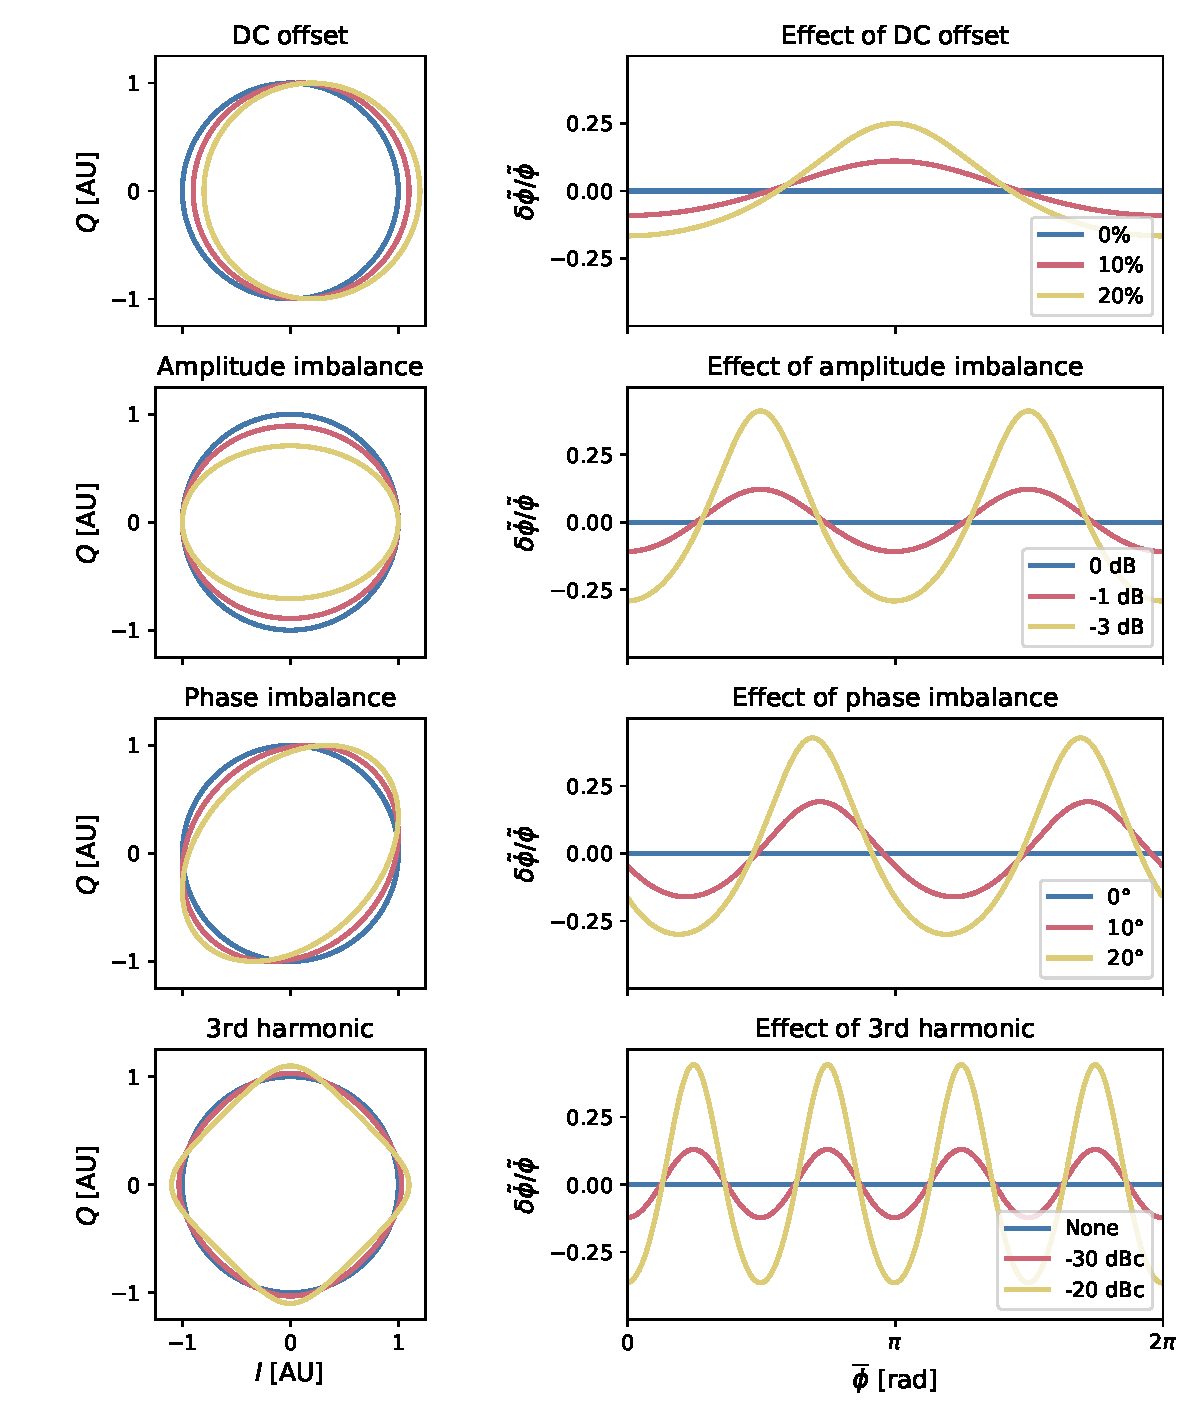
\includegraphics[width = \textwidth]{%
    Chapters/DesignConsiderations/figs/demodulator_imperfections.pdf}
  \caption[Effects of demodulator imperfections]{%
    Demodulator imperfections produce errors in the measured phase.
    The left column displays the Lissajous curves
    that result from plotting
    the quadrature $Q$ vs.\ in-phase $I$ signals, while
    the right column plots the relative error
    $\delta\tilde{\phi} / \tilde{\phi}$
    in the measured fluctuating phase
    as a function of the equilibrium phase $\bar{\phi}$.
    Each row examines a different demodulator imperfection.
  }
  \label{fig:DesignConsiderations:effects_of_demodulator_imperfections}
\end{figure}


\section{Intensity considerations}
Ideally, a photovoltaic detector produces an output voltage
\begin{equation}
  V(t) = \mathcal{R}_0 \cdot I(t),
\end{equation}
where $\mathcal{R}_0$ is the detector responsivity and
$I(t)$ is the incident optical intensity.
However, every real-world detector has a saturation intensity $I_{\text{sat}}$
beyond which the output voltage ceases to be a linear function
of the incident optical intensity; that is,
the detector responsivity has an intensity dependence $\mathcal{R}(I)$, and
the detector voltage can be more generally written as
\begin{equation}
  V(t) = \mathcal{R}\left( I(t) \right) \cdot I(t).
\end{equation}
Here, $\mathcal{R}(I)$ is an arbitrary monotonically increasing function
of the incident optical intensity $I$.
Despite the potentially nonlinear response,
the detector voltage remains periodic in $2 \pi / \Delta \omega_0$ and
can be expanded in a Fourier series as
\begin{equation}
  V(t)
  =
  V_0
  +
  \sum_{n = 1}^{\infty}
  V_n \cos\left( n \Delta \omega_0 t + \theta_n \right),
\end{equation}
where $V_n$ and $\theta_n$ are the amplitude and phase, respectively,
of the $n\ts{th}$ harmonic.
Thus, a nonlinear detector response produces
higher-order harmonics in the signal.
In general, $V_n$ and $\theta_n$ can vary in time,
producing sidebands about each harmonic.
Provided the bandwidth of these fluctuations is sufficiently low,
there will be no spectral overlap
between the sidebands of adjacent harmonics, and
bandpass filtering the detector signal about $\Delta \omega_0$ yields
\begin{equation}
  V(t) \approx V_1 \cos[\Delta \omega_0 t + \theta_1(t)]
\end{equation}
with $\theta_1(t) = \phi(t)$, where
$\phi(t)$ is the optical phase shift
between the plasma and reference arms of the interferometer.
However, for fluctuations with sufficiently high bandwidth
(e.g.\ $\omega \sim \Delta\omega_0 / 2$),
the sidebands of adjacent harmonics begin to overlap,
potentially corrupting the phase measurement.

\begin{figure}
  \centering
  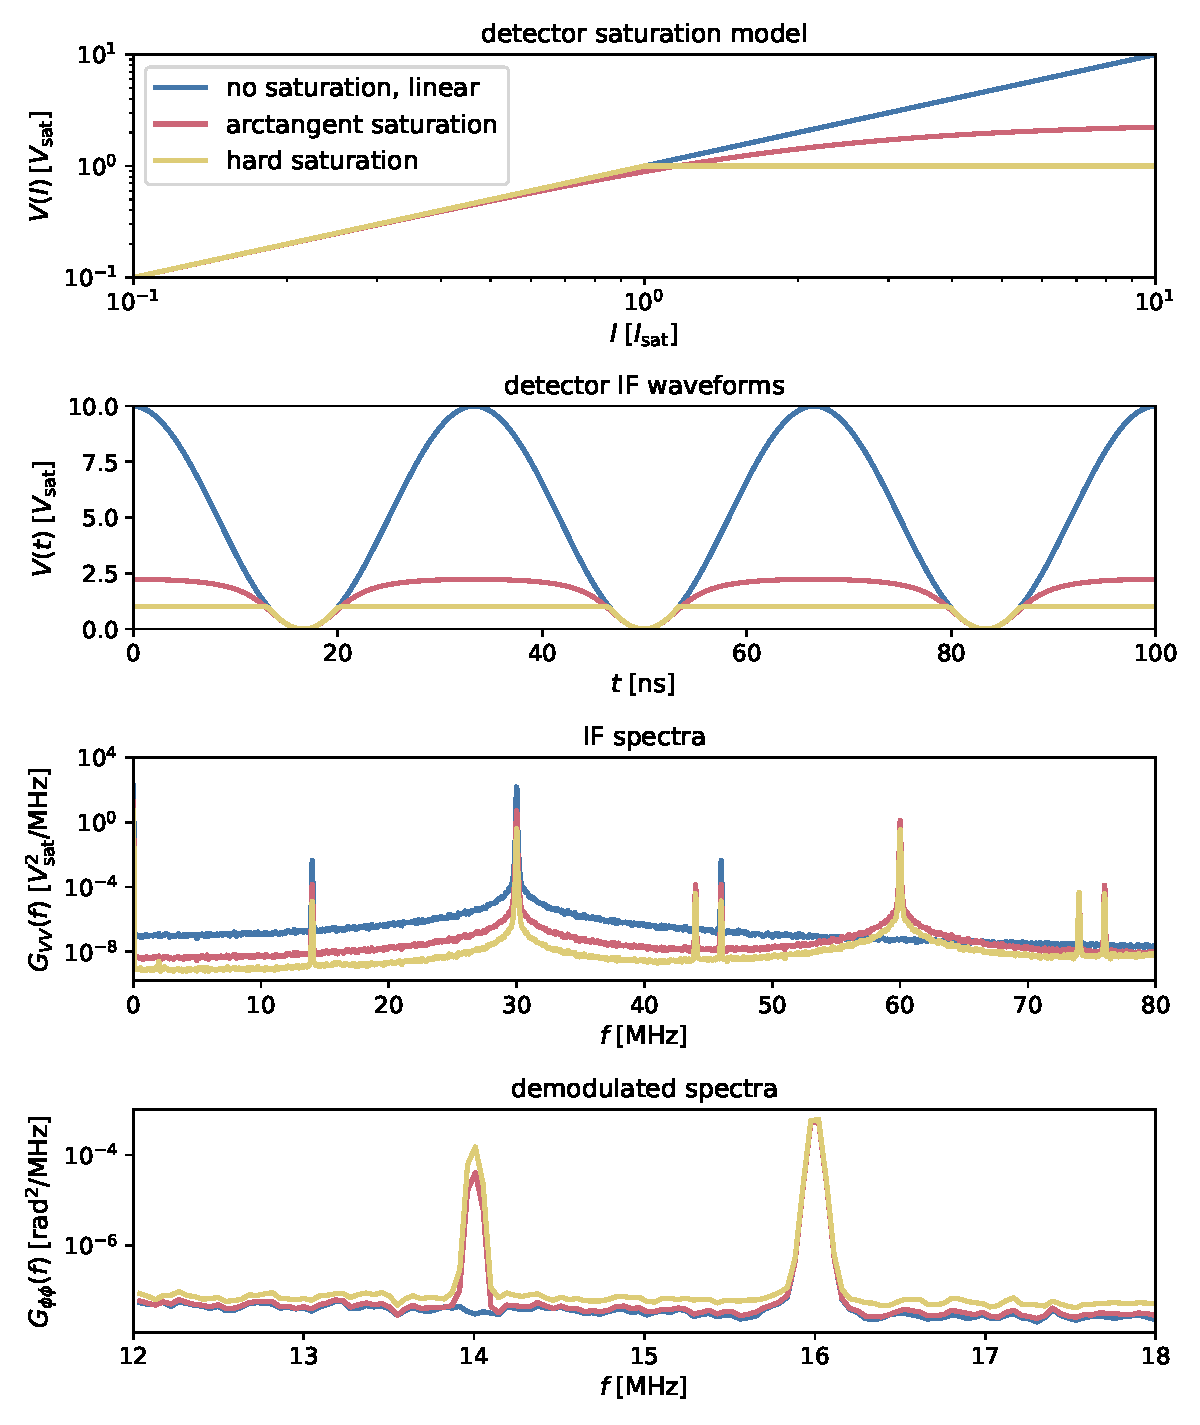
\includegraphics[width = \textwidth]{%
    Chapters/DesignConsiderations/figs/nonlinear_heterodyne_detection.pdf}
  \caption[Heterodyne detection beyond saturation intensity]{%
    Heterodyne detection beyond the saturation intensity.}
\label{fig:DesignConsiderations:nonlinear_heterodyne_detection}
\end{figure}

\begin{itemize}
  \item Transfer function in context of Ch.~2 when in saturation?
\end{itemize}


\bibliographystyle{plainurl}
\bibliography{references}
